%% Application à des données réelles
% le Sweaveopt


\chapter{Application à des données réelles}
\label{chap:application} 

\section{Analyse de données}

Pour mettre en application l'approche proposée par \cite{chavez2016extreme}, deux jeux de données du paquetage \texttt{CASdatasets} sont utilisés. Soit \texttt{auscathist} et \texttt{nzcathist}. Ces données représentent respectivement l'historique des catastrophes naturelles pour l'Australie ainsi que pour la Nouvelle-Zélande. Les deux jeux de données contiennent également différentes statistiques de ces catastrophes. Voici une liste des variables disponibles:
\begin{itemize}
\item \texttt{Year}: l'année d'occurence de la catastrophe.
\item \texttt{Quarter}: le trimestre d'occurence de la catastrophne.
\item \texttt{Date}: la date d'occurence complète de la catastrophe.
\item \texttt{FirstDay}: la date de la première journée d'occurence de la catastrophe.
\item \texttt{LastDay}: la date de la dernière journée de la catastrophe (seulement disponible pour l'Australie).
\item \texttt{Event}: une description de la catastrophe.
\item \texttt{Type}: le type de catastrophe.
\item \texttt{Location}: une description du lieu de la catastrophe.
\item \texttt{OriginalCost}: coût original de la catastrophe en millions de \textit{AUD} ou \textit{NZD}.
\item \texttt{NormCost2011}: coût normalisé en millions de dollars de 2011 (inflation, richesse et population).
\item \texttt{NormCost2014}: coût normalisé en millions de dollars de 2014 (inflation, richesse et population).
\end{itemize}
\

Les tables \ref{tab:3.1} et \ref{tab:3.2} contiennent un résumé statistique des données australiennes. Les tables \ref{tab:3.3} et \ref{tab:3.4} contiennent le même type de résumé pour la Nouvelle-Zélande.


% latex table generated in R 3.6.1 by xtable 1.8-4 package
% Mon Dec  2 15:08:45 2019
\begin{table}[ht]
\centering
\begin{tabular}{cccccccc}
  \hline
 & Mean & Std.Dev & Min & Median & Max & N.Valid & Pct.Valid \\ 
  \hline
NormCost2011 & 254 & 589 & 2 & 66 & 4296 & 190 & 92 \\ 
  NormCost2014 & 288 & 639 & 2 & 77 & 4606 & 206 & 100 \\ 
  OriginalCost & 104 & 295 & 1 & 15 & 2388 & 206 & 100 \\ 
  Quarter & 2 & 1 & 1 & 2 & 4 & 206 & 100 \\ 
  Year & 1995 & 12 & 1967 & 1998 & 2014 & 206 & 100 \\ 
   \hline
\end{tabular}
\caption{Résumé statistique des variables numériques pour l'Australie} 
\label{tab:3.1}
\end{table}% latex table generated in R 3.6.1 by xtable 1.8-4 package
% Mon Dec  2 15:08:45 2019
\begin{table}[ht]
\centering
\begin{tabular}{cccccc}
  \hline
 & Freq & \% Valid & \% Valid Cum. & \% Total & \% Total Cum. \\ 
  \hline
Bushfire & 26 & 13 & 13 & 13 & 13 \\ 
  Cyclone & 33 & 16 & 29 & 16 & 29 \\ 
  Earthquake & 4 & 2 & 31 & 2 & 31 \\ 
  Flood & 25 & 12 & 43 & 12 & 43 \\ 
  Flood, Storm & 27 & 13 & 56 & 13 & 56 \\ 
  Hailstorm & 33 & 16 & 72 & 16 & 72 \\ 
  Other & 3 & 1 & 73 & 1 & 73 \\ 
  Storm & 54 & 26 & 100 & 26 & 100 \\ 
  Tornado & 1 & 0 & 100 & 0 & 100 \\ 
  $<$NA$>$ & 0 &  &  & 0 & 100 \\ 
  Total & 206 & 100 & 100 & 100 & 100 \\ 
   \hline
\end{tabular}
\caption{Distribution du Type de catastrophe pour l'Australie} 
\label{tab:3.2}
\end{table}
% latex table generated in R 3.6.1 by xtable 1.8-4 package
% Mon Dec  2 15:08:45 2019
\begin{table}[ht]
\centering
\begin{tabular}{cccccccc}
  \hline
 & Mean & Std.Dev & Min & Median & Max & N.Valid & Pct.Valid \\ 
  \hline
NormCost2011 & 17.169 & 40.885 & 0.010 & 5.270 & 371.120 & 129.000 & 88.966 \\ 
  NormCost2014 & 137.777 & 1437.470 & 0.000 & 5.870 & 17320.680 & 145.000 & 100.000 \\ 
  OriginalCost & 124.591 & 1369.525 & 0.000 & 3.500 & 16500.000 & 145.000 & 100.000 \\ 
  Quarter & 2.262 & 1.143 & 1.000 & 2.000 & 4.000 & 145.000 & 100.000 \\ 
  Year & 1999.448 & 10.674 & 1968.000 & 2001.000 & 2014.000 & 145.000 & 100.000 \\ 
   \hline
\end{tabular}
\caption{Résumé statistique des variables numériques pour la Nouvelle-Zélande} 
\label{tab:3.3}
\end{table}% latex table generated in R 3.6.1 by xtable 1.8-4 package
% Mon Dec  2 15:08:45 2019
\begin{table}[ht]
\centering
\begin{tabular}{cccccc}
  \hline
 & Freq & \% Valid & \% Valid Cum. & \% Total & \% Total Cum. \\ 
  \hline
Cyclone & 4 & 3 & 3 & 3 & 3 \\ 
  Earthquake & 7 & 5 & 8 & 5 & 8 \\ 
  Flood & 58 & 40 & 48 & 40 & 48 \\ 
  Flood, Storm & 9 & 6 & 54 & 6 & 54 \\ 
  Hailstorm & 8 & 6 & 59 & 6 & 59 \\ 
  Other & 10 & 7 & 66 & 7 & 66 \\ 
  Power outage & 2 & 1 & 68 & 1 & 68 \\ 
  Storm & 32 & 22 & 90 & 22 & 90 \\ 
  Tornado & 11 & 8 & 97 & 8 & 97 \\ 
  Weather & 4 & 3 & 100 & 3 & 100 \\ 
  $<$NA$>$ & 0 &  &  & 0 & 100 \\ 
  Total & 145 & 100 & 100 & 100 & 100 \\ 
   \hline
\end{tabular}
\caption{Distribution du Type de catastrophe pour la Nouvelle-Zélande} 
\label{tab:3.4}
\end{table}

Pour chaque jeu de données, une nouvelle variable du montant de catastrophe est créée à partir de la variable \texttt{NormCost2014} (\texttt{CostUS2019}). Cette nouvelle variable représente le coût ajusté au niveau du 30 juin 2019 en considérant l'indice du prix à la consommation de chaque pays et le coût est également converti en dollar américain. La table \ref{tab:3.5} contient les chiffres utilisés \footnote{https://www.rateinflation.com/consumer-price-index  \newline https://www.exchange-rates.org/Rate/AUD/USD/6-30-2019}.

% latex table generated in R 3.6.1 by xtable 1.8-4 package
% Mon Dec  2 15:08:45 2019
\begin{table}[ht]
\centering
\begin{tabular}{cccc}
  \hline
 & IPC 2014 & IPC 2019 & Taux de change 2019 \\ 
  \hline
AUS & 105.9000 & 114.8000 & 0.7031 \\ 
  NZ & 974.7000 & 1039.0000 & 0.6722 \\ 
   \hline
\end{tabular}
\caption{Valeurs utilisées pour CostUS2019} 
\label{tab:3.5}
\end{table}\

Étant donné que les deux jeux de données sont très semblables, ceux-ci sont regroupés en un seul jeu de données et une variable \texttt{Country} est rajoutée. Étant donné le nombre limité de données disponibles et pour rendre l'analyse pertinente et possible, seulement les variables \texttt{CostUS2019}, \texttt{Year}, \texttt{Country} et \texttt{Type} sont conservées. Les figures \ref{fig:3.1}, \ref{fig:3.2}, \ref{fig:3.3} ainsi que la table \ref{tab:3.6} résument bien le jeu de données final utilisé pour commencer l'analyse.


\begin{figure}[h]
\begin{center}
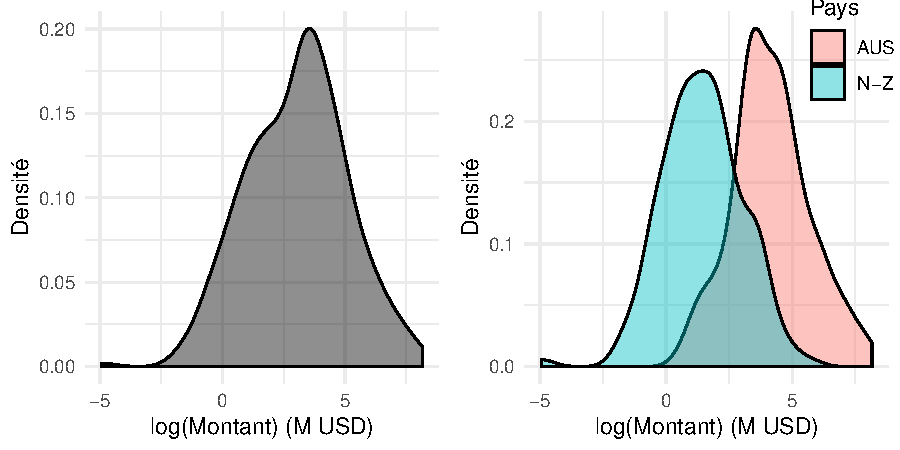
\includegraphics{images/fig-005}
\end{center}
\caption{Densité du logarithme du montant des catastrophes}
\label{fig:3.1}
\end{figure}

\begin{figure}[h]
\begin{center}
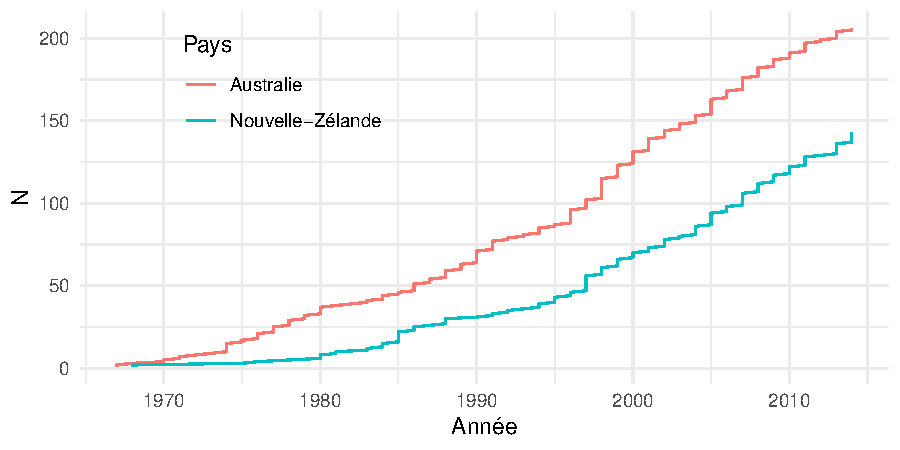
\includegraphics{images/fig-006}
\end{center}
\caption{Nombre cumulatif de catastrophes par pays}
\label{fig:3.2}
\end{figure}


\begin{figure}[h]
\begin{center}
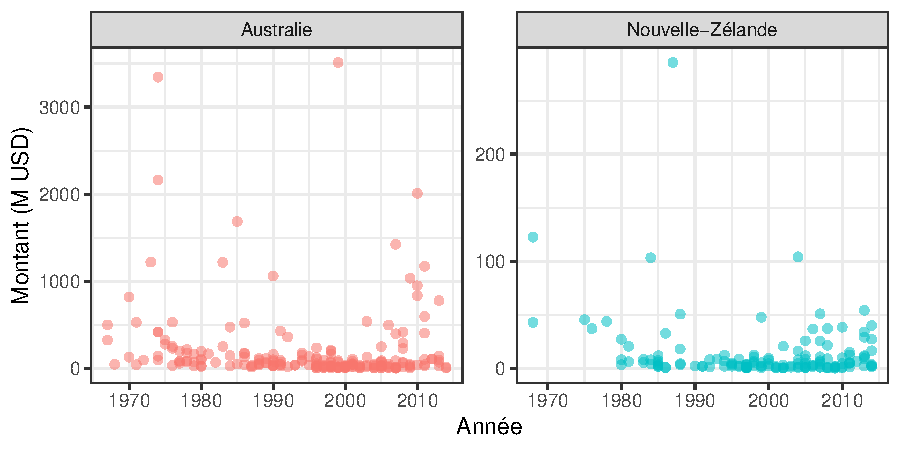
\includegraphics{images/fig-007}
\end{center}
\caption{Évolution des catastrophes par pays}
\label{fig:3.3}
\end{figure}   

% latex table generated in R 3.6.1 by xtable 1.8-4 package
% Mon Dec  2 15:08:47 2019
\begin{table}[ht]
\centering
\begin{tabular}{cccccccc}
  \hline
Type & N & Moyenne & Écart & Minimum & Médiane & Q3 & Maximum \\ 
  \hline
Bushfire & 26 & 143 & 259 & 7 & 39 & 134 & 1217 \\ 
  Cyclone & 37 & 325 & 675 & 2 & 88 & 217 & 3343 \\ 
  Earthquake & 9 & 56 & 91 & 0 & 25 & 47 & 286 \\ 
  Flood & 83 & 62 & 230 & 0 & 5 & 39 & 2010 \\ 
  Flood, Storm & 36 & 54 & 79 & 1 & 24 & 71 & 414 \\ 
  Hailstorm & 41 & 274 & 606 & 0 & 75 & 235 & 3511 \\ 
  Other & 12 & 121 & 296 & 2 & 6 & 50 & 1035 \\ 
  Power outage & 2 & 6 & 6 & 1 & 6 & 8 & 11 \\ 
  Storm & 86 & 97 & 228 & 0 & 28 & 57 & 1424 \\ 
  Tornado & 12 & 7 & 13 & 0 & 3 & 7 & 47 \\ 
  Weather & 4 & 11 & 11 & 2 & 6 & 13 & 27 \\ 
   \hline
\end{tabular}
\caption{Résumé statistique des montants (M USD) de catastrophes par Type} 
\label{tab:3.6}
\end{table}
\clearpage
\section{Approche classique}

Avant d'essayer la nouvelle méthode proposée, les méthodes classiques présentées à au chapitre \ref{chap:notions} sont appliquées pour être en mesure d'évaluer la valeur de la nouvelle méthode. Plus spécifiquement, l'approche \textit{POT} présentée à la section \ref{sec:pot} est appliquée dans la présente section étant donné que c'est ce type de modèle qui est appliqué dans les prochaines sections. À noter que les différents calculs de cette section nécessitant des techniques numériques sont faits avec le paquetage \texttt{ismev}. L'approche ici est donc de prendre l'ensemble des données, de choisir un seuil $u$ approprié et d'estimer les paramètres de la loi Pareto généralisée avec les excès de seuil, le tout en tenant compte d'aucunes variables exogènes. Comme mentionné, la première étape de cette méthodologie est le choix de la valeur du seuil $u$. La première méthode demande de tracer le \textit{mean residual plot} dont les points mentionnés dans l'équation \ref{eq:1.2.5}. Après un certaine valeur $u$ pour lequel la distribution est appropriée, le graphique devrait être linéaire en $u$. La figure \ref{fig:3.4} montre que déjà à partir de petites valeurs, cette conditon est respectée, il est ensuite difficile, voire subjectif de choisir une valeur précise. Ici, le graphique suggère de sélectionner une valeur entre 0 et 10.
\begin{figure}[h]
\begin{center}
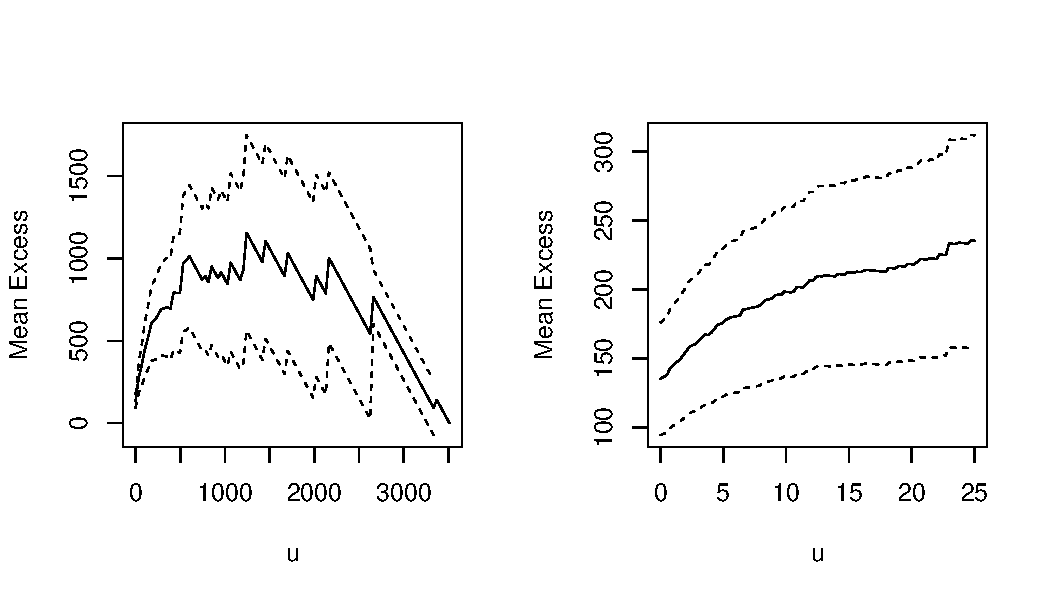
\includegraphics{images/fig-009}
\end{center}
\caption{\textit{Mean residual plot}}
\label{fig:3.4}
\end{figure}

La deuxième méthode mentionnée à la section \ref{sec:pot} propose d'estimer les paramètres du modèle pour différentes valeurs de $u$. Comme expliqué dans cette section, $\sigma^*$ et $\xi$ devraient rester constants au-delà de $u_0$. La figure \ref{fig:3.5} montre des résulats plus concluants que la figure \ref{fig:3.4}. En effet, les valeurs de $\sigma^*$ et de $\xi$ deviennent constantes environ à $u=10$. L'analyse des deux différentes techniques de sélection de seuil mènent donc à une sélection de $u=10$. Environ 64\% des données dépassent ce seuil, un bon nombre de données est donc utile pour la modélisation des excès.
\begin{figure}[h]
\begin{center}
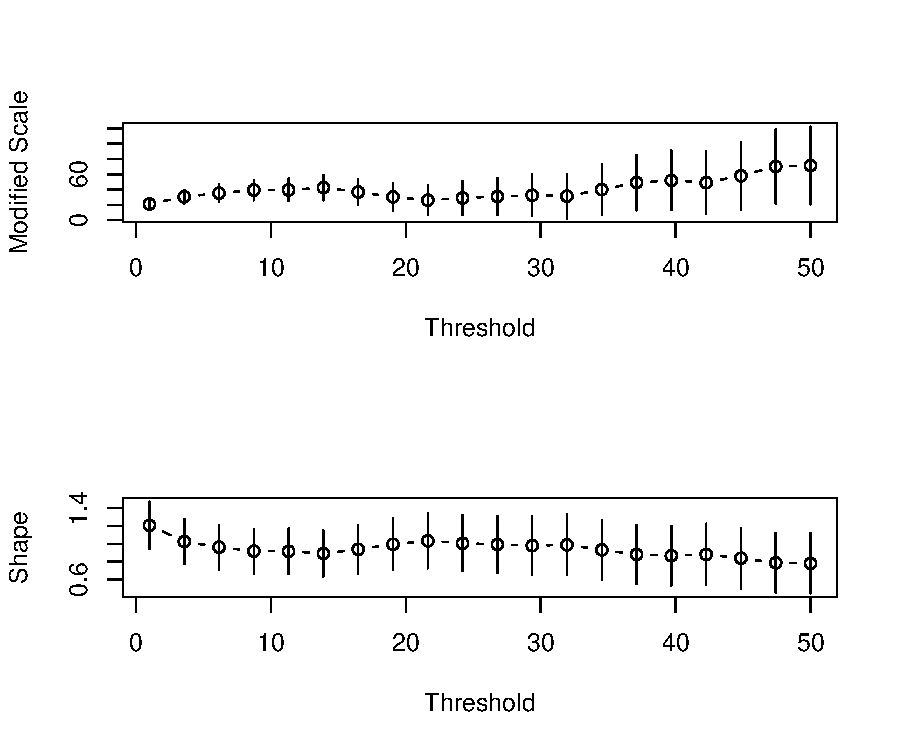
\includegraphics{images/fig-010}
\end{center}
\caption{Estimation des paramètres du modèle pour différents seuils}
\label{fig:3.5}
\end{figure}

Après avoir sélectionné le seuil, il faut ensuite estimer les paramètres de la loi Pareto généralisée avec la méthode du maximum de vraisemblance. Les différents détails de ce calcul se trouvent dans les équations \ref{eq:1.2.6} et \ref{eq:1.2.7}. Voici les résultats obtenus avec un intervalle de confiance de 95 \%.

\begin{equation*}
\begin{gathered}
(\hat\sigma,\hat\xi) = (49.329951;\ 0.941132)\\
\ell(\hat\sigma,\hat\xi) = -1308.013\\
\text{Var}(\hat\sigma) = 41.9446912\\
\text{Var}(\hat\xi) = 0.01673518
\end{gathered}
\end{equation*}
\

\begin{equation*}
\begin{gathered}
\hat\zeta_u = 0.6418338\\
\text{Var}(\hat\zeta_u) = 0.000658691
\end{gathered}
\end{equation*}
\

\begin{equation*}
\begin{gathered}
IC_{\hat\sigma} = (36.6362993;\ 62.023603)\\
IC_{\hat\xi} = (0.6875822;\ 1.194682)\\
IC_{\hat\zeta_u} = (0.5915314;\ 0.6921362)
\end{gathered}
\end{equation*}
\

Suite aux résultats obtenus, les graphiques de validation mentionnés à la section \ref{sec:pot} peuvent être tracés pour juger de la qualité du modèle. La figure \ref{fig:3.6} montre des résultats qui ne sont pas désastreux, mais qui sont loin d'être concluants en ce qui concerne l'ajustement des données au modèle proposé dans la présente section. Le graphique \textit{P-P} est tout de même adéquat, mais les trois autres graphiques sont loins de l'être. Les graphiques \textit{Q-Q} et celui de la densité obtenue montrent que le modèle représentent mal les données utilisées et le graphique des niveaux de retour montre que dès que la période de retour est un peu élevé, le niveau obtenu est extrêmement volatile. 
\


Pour conclure, le modèle proposé dans cette section représente un modèle de base qui considère toutes les données de la manière sans égard aux informations supplémentaires disponibles par rapport aux montants des catastrophes. Il n'est donc pas surprenant de voir que cette approche n'est pas tout à fait adéquate dans le cas présent, mais reste que cette approche est viable, rapide et peut être une bonne solution lorsque seulement les montants sont disponibles. Il est également important de savoir que le modèle testé dans cette section est la base de tous autres modèles plus avancés, tous comme les modèles qui seront testés aux prochaines sections.
\begin{figure}[h]
\begin{center}
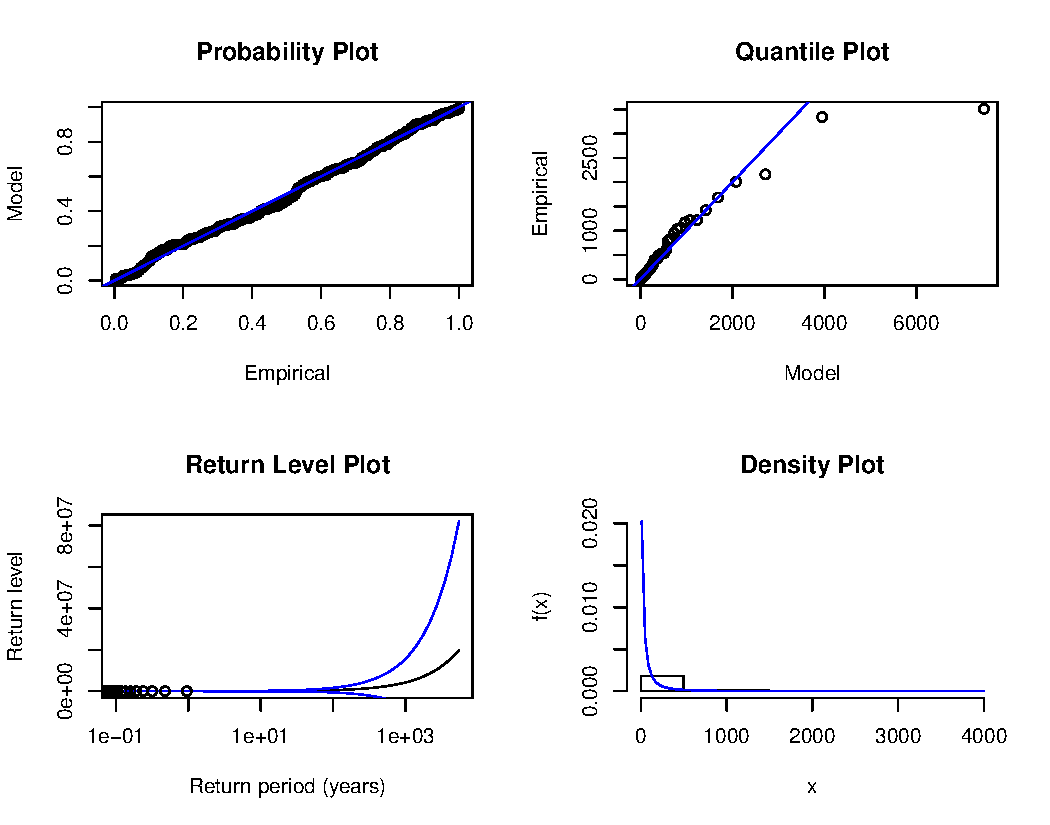
\includegraphics{images/fig-011}
\end{center}
\caption{Graphiques de validation du modèle}
\label{fig:3.6}
\end{figure}


\clearpage
\section{Approche dynamique à deux variables}
\label{sec:3.3}

Cette section applique la méthodologie et le modèle proposés au chapitre \ref{chap:article} avec deux variables, l'année et le pays. On considère donc une variable numérique de temps ainsi qu'une variable catégorique à deux niveaux. Seulement deux variables sont initialemment utilisées étant donné que c'est ce que l'article étudié utilise pour ilustrer la méthode. De plus, étant donné le nombre limité de données disponibles, il est préférable de ne pas commencer avec un nombre de sous-groupes trop élevés. Une troisième variable sera considérée à la section \ref{sec:3.4}. Avant même de commencer, les figures \ref{fig:3.1} et \ref{fig:3.2} suggèrent que les paramètres du modèles devraient bel et bien varier entre les deux pays et à travers le temps. Dans le cadre de la modélisation, seulement l'ajustement du paramètre $\rho$ est inclu dans le rapport, voir \ref{eq:2.2.13}. Un seuil de valeur 10 M USD est toujours utilisé, voir les figures \ref{fig:3.4} et \ref{fig:3.5}. 
\\

Premièrement, le paramètre $\rho$ du modèle est ajusté aux données. Après avoir statistiquement comparé les différents modèles, le modèle sélectionné pour $\hat\rho$ dépend du pays et du temps et a la forme suivante:
\begin{equation}\label{eq:3.3.1}
\log\Bigg(\frac{\hat\rho(x,t)}{1-\hat\rho(x,t)}\Bigg) = \hat{f}_\rho(pays) + \hat{h}^{(2)}_\rho(annee)
\end{equation}
où ${h}^{(\text{Df})}$ représente une spline naturelle quadratique avec $\text{Df}$ degrés de liberté.
\\


Voici une représentation graphique des résultats obtenus.
\begin{figure}[h]
\begin{center}
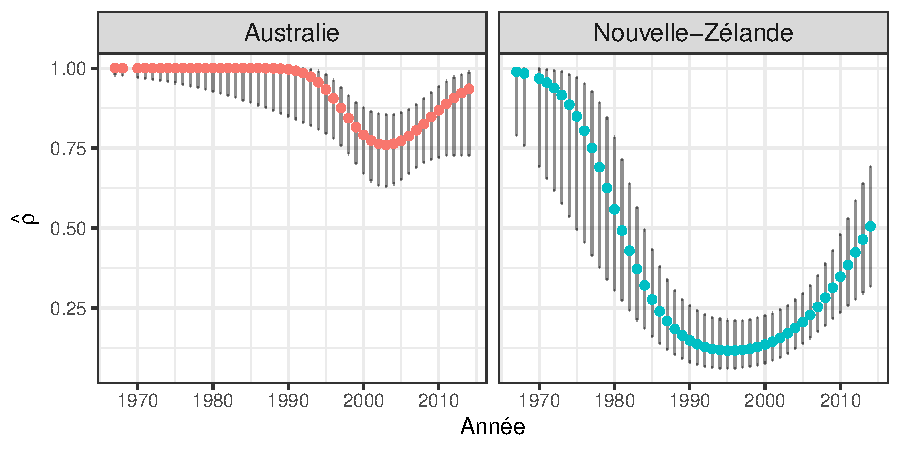
\includegraphics{images/fig-013}
\end{center}
\caption{Prédictions du taux d'excès de seuil avec intervalles de confiance à 95\%}
\label{fig:3.7}
\end{figure}

La figure \ref{fig:3.7} indique qu'il y a bel et bien une différence entre les pays et à travers le temps. Plus spécifiquement, les catastrophes australiennes dépassent beaucoup plus souvent le seuil de 10 millions et la figure indique également un paramètre élevé et constant pendant quelques années pour ensuite observé une diminution de celui-ci pour que finalement celui-ci remonte à un certain niveau.
\\

Ensuite, les paramètres de la loi Pareto généralisée sont ajustés aux données. Après avoir statistiquement comparé les différents modèles, le modèle sélectionné pour $\hat\xi$ dépend du pays et non du temps et a la forme suivante:
\begin{equation}\label{eq:3.3.2}
\hat\xi(x,t) = \hat{f}_\xi(pays)
\end{equation}

De son côté, le modèle sélectionné pour $\hat\beta$ dépend du pays et du temps et a la forme suivante:
\begin{equation}\label{eq:3.3.3}
\hat\beta(x,t) = \hat{f}_\beta(pays) + \hat{h}^{(3)}_\beta(annee)
\end{equation}



Les figures \ref{fig:3.8} et \ref{fig:3.9} présentent une représentation graphique des résultats obtenus pour les deux paramètres.
\begin{figure}[h]
\begin{center}
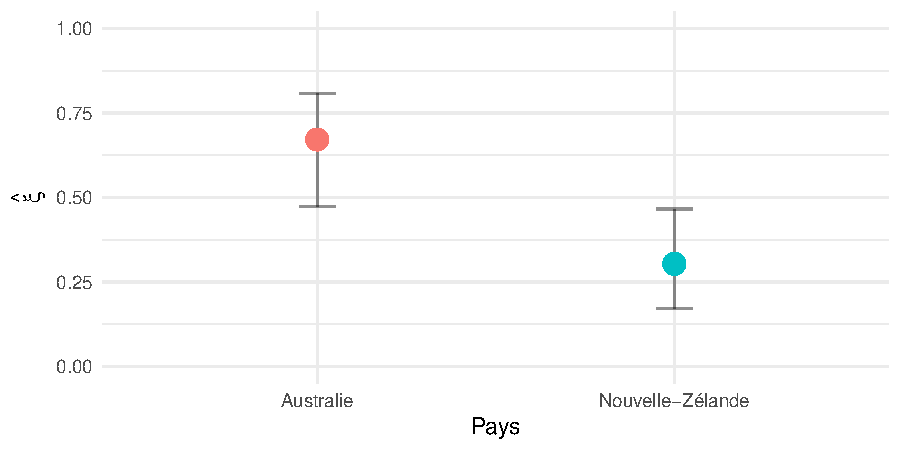
\includegraphics{images/fig-015}
\end{center}
\caption{Prédictions du paramètre $\xi$ avec intervalles de confiance à 95\%}
\label{fig:3.8}
\end{figure}

La figure \ref{fig:3.8} montre qu'il y a bel et bien une différence entre les deux pays et que cette différence est très importante. Le fait que le paramètre de l'Australie soit plus élevé fait du sens, car la distribution des catastrophes australiennes a une queue plus épaisse que celle des catastrophes de la Nouvelle-Zélande. 
\\

\begin{figure}[h]
\begin{center}
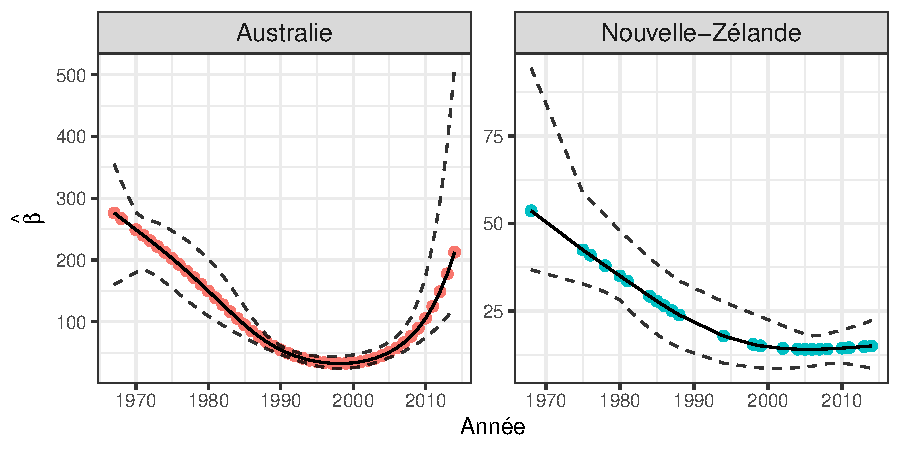
\includegraphics{images/fig-016}
\end{center}
\caption{Prédictions du paramètre $\beta$ avec intervalles de confiance à 95\%}
\label{fig:3.9}
\end{figure}

La figure \ref{fig:3.9} montre bien que les deux variables sélectionnées ont bel et bien un impact sur le paramètre $\beta$. Tout comme avec $\xi$, il est logique que les paramètres de la Nouvelle-Zélande soient inférieurs que ceux de l'Australie tout simplement parce que les pertes sont généralement plus élevées, voir la figure \ref{fig:3.1}. La figure montre également que, de façon générale, le paramètre dimiunue avec le temps.
\\

Même si les paramètres du modèle sont maintenant obtenus, il est important de vérifier l'adéquation du modèle avant d'effectuer n'importe quelle inférence. Comme l'explique l'équation \ref{eq:2.2.12}, une validation possible est de vérifier si les $r_i$ se comportent comme des variables aléatoires indépendantes suivant une loi exponentielle standards. Le graphique \textit{Q-Q} de cette loi est donc tracé à la figure \ref{fig:3.10}.

La figure montre que la calibration du modèle n'est pas tout si mal et même bonne dans l'ensemble. Le graphique n'est pas catastrophique et tout de même mieux que celui de la figure \ref{fig:3.6}. Peut-être que l'ajout d'une troisième variable à la section \ref{sec:3.4} va améliorer la qualité du modèle obtenu.
\\

Ensuite, à l'aide de l'équation \ref{eq:2.2.13}, les différentes $\widehat{\text{VaR}_{0.99}}$ peuvent être calculées. La figure \ref{fig:3.11} montre les résultats. 
\begin{figure}[h]
\begin{center}
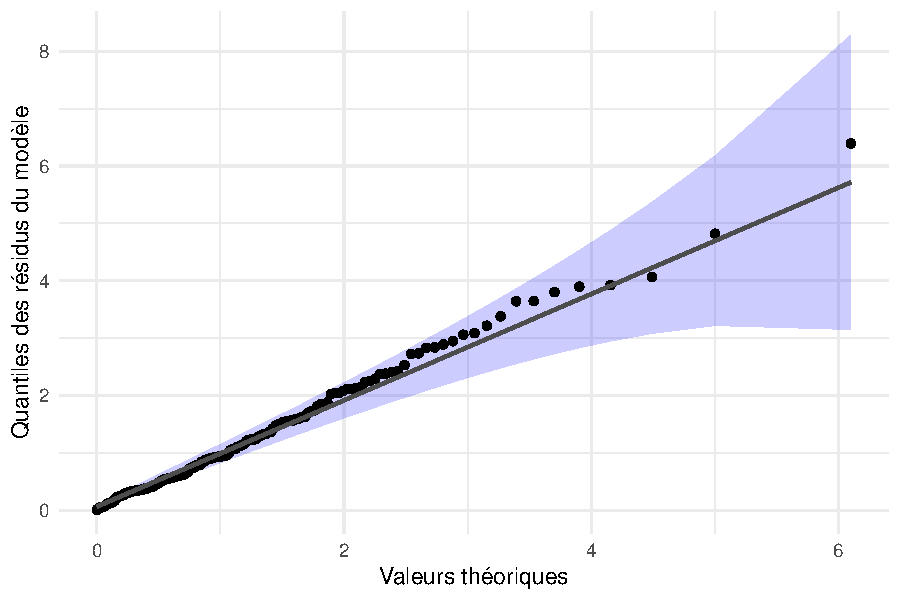
\includegraphics{images/fig-018}
\end{center}
\caption{Graphique \textit{Q-Q} de $\text{Exp}(1)$}
\label{fig:3.10}
\end{figure}

\begin{figure}[h]
\begin{center}
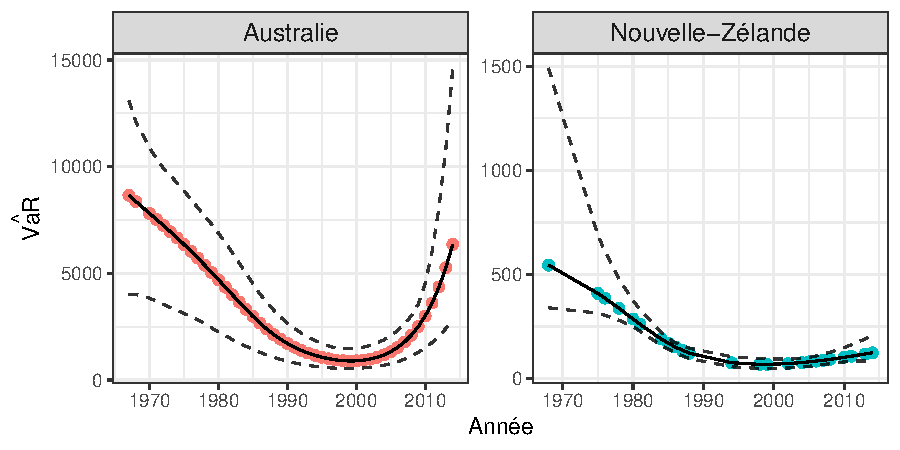
\includegraphics{images/fig-019}
\end{center}
\caption{$\widehat{\text{VaR}_{0.99}}$ avec intervalles de confiance à 95\%}
\label{fig:3.11}
\end{figure}

Il est logique de voir que la mesure de risque dépend du temps et du pays car celle-ci est obtenue avec les paramètres estimés. Tout comme avec les paramètres, il est logique que les valeurs obtenues pour la Nouvelle-Zélande soient inférieurs que celles de l'Australie tout simplement parce que les pertes sont généralement plus élevées pour l'Australie.
\\

C'est ce qui conclut cette section. La méthodologie proposée par les auteurs fonctionne et donnent les résultats escomptés lorque le temps ainsi qu'une variable catégorique sont considérés. Le modèle final obtenu n'est pas parfait, mais est tout de même une amélioration du modèle classique vu à la section \ref{sec:pot}.


\clearpage
\section{Approche dynamique à trois variables}
\label{sec:3.4}

Dans cette section, la même procédure que la section \ref{sec:3.3} est employée, mais la variable représentant le type de catastrophes est maintenant disponible. Un seuil de 10 M USD est toujours utilisé. Il y a 11 types différents dans les données. Une démarche complète de modélisation a été faite avec tous les types non regroupés, mais étant donné le nombre limité de données, les résultats ne furent pas concluants et les détails de ce modèle ne sont pas incluts dans ce rapport. Pour être en mesure de travailler avec cette troisième variable, un regroupement des types a dû être fait. La table \ref{tab:3.7} présente un résumé de ce regroupement. Sans même commencer la modélisation, la table \ref{tab:3.6} montre que le type de catastrophes va probablement s'avérer significatif pour les différents paramètres du modèle étant donnée que la distribution du montant de catastrophe varie beaucoup entre les différents types. 


% latex table generated in R 3.6.1 by xtable 1.8-4 package
% Mon Dec  2 15:11:12 2019
\begin{table}[ht]
\centering
\begin{tabular}{cc}
  \hline
Type & Type2 \\ 
  \hline
Bushfire & Bushfire \\ 
  Hailstorm & Hailstorm \\ 
  Cyclone & Cyclone \\ 
  Flood & Flood, Storm \\ 
  Flood, Storm & Flood, Storm \\ 
  Storm & Flood, Storm \\ 
  Other & Other \\ 
  Tornado & Other \\ 
  Earthquake & Other \\ 
  Weather & Other \\ 
  Power outage & Other \\ 
   \hline
\end{tabular}
\caption{Regroupement des types de catastrophes} 
\label{tab:3.7}
\end{table}
Tout comme lors de section précédente, le paramètre $\rho$ du modèle est le premier à être ajusté aux données. Après avoir statistiquement comparé les différents modèles, le modèle sélectionné pour $\hat\rho$ dépend du pays, du type et du temps et a la forme suivante:
\begin{equation}\label{eq:3.4.1}
\log\Bigg(\frac{\hat\rho(x,t)}{1-\hat\rho(x,t)}\Bigg) = \hat{f}_\rho(pays) + \hat{f}_\rho(type) + \hat{h}^{(2)}_\rho(annee)
\end{equation}

La figure \ref{fig:3.12} montre les résultats pour l'Australie et la figure ref{fig:3.13} montre ceux pour la Nouvelle-Zélande.
\\



\begin{figure}[h]
\begin{center}
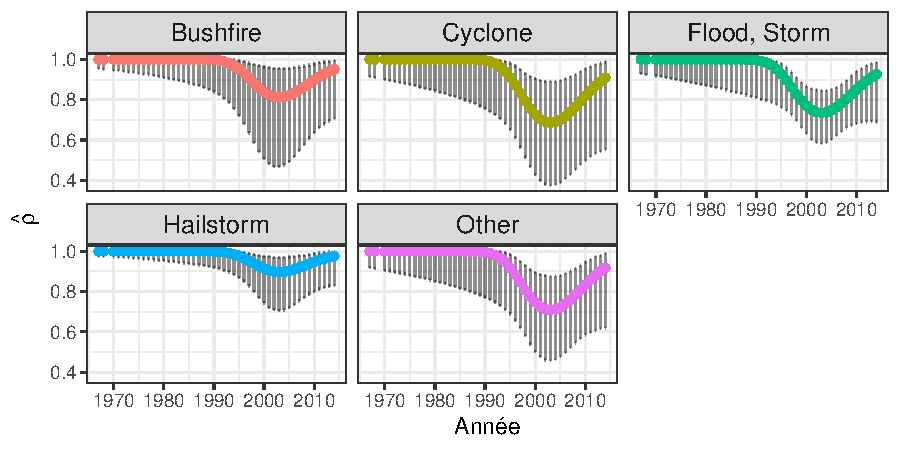
\includegraphics{images/fig-023}
\end{center}
\caption{Prédictions du paramètre $\rho$ pour l'Australie avec intervalles de confiance à 95\%}
\label{fig:3.12}
\end{figure}

\begin{figure}[h]
\begin{center}
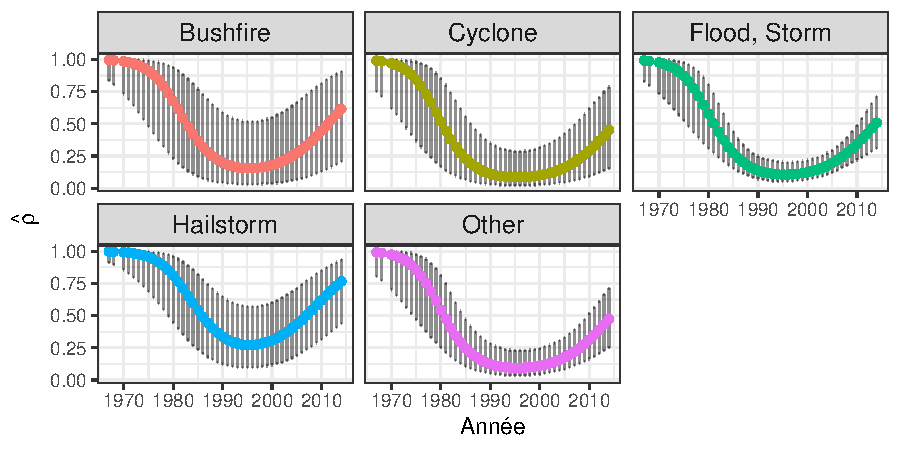
\includegraphics{images/fig-024}
\end{center}
\caption{Prédictions du paramètre $\rho$ pour la Nouvelle-Zélande avec intervalles de confiance à 95\%}
\label{fig:3.13}
\end{figure}

Les deux figures montrent que, comme dans la section précédente, il est clair que le paramètre est différent entre les deux pays et que celui-ci dépend du temps. De plus, même si cela est moins significatif que les pour les autres variables, les figures montrent également que le type de catastrophes est important pour la détermination du paramètre. Les courbes sont semblables par pays, mais le type amène une certaine translation verticale de la courbe. Cependant, on peut voir que les intervalles de confiance sont plus larges que ceux de la figure \ref{fig:3.7} étant donné qu'il y a maintenant moins de données par sous-groupes de variables.
\\

Suivant à nouveau la même démarche que la section précédente, les paramètres de la loi Pareto généralisée sont ajustés aux données. Après avoir statistiquement comparé les différents modèles, le modèle sélectionné pour $\hat\xi$ dépend du pays, du type et non du temps et a la forme suivante:
\begin{equation}\label{eq:3.4.2}
\hat\xi(x,t) = \hat{f}_\xi(pays) + \hat{f}_\xi(type)
\end{equation}

De son côté, le modèle sélectionné pour $\hat\beta$ dépend du pays, du type et du temps et a la forme suivante:
\begin{equation}\label{eq:3.4.3}
\hat\beta(x,t) = \hat{f}_\beta(pays) + \hat{f}_\xi(type) + \hat{h}^{(4)}_\beta(annee)
\end{equation}


Les figures \ref{fig:3.14}, \ref{fig:3.15} et \ref{fig:3.16} présentent une représentation graphique des résultats obtenus pour les deux paramètres.
\begin{figure}[h]
\begin{center}
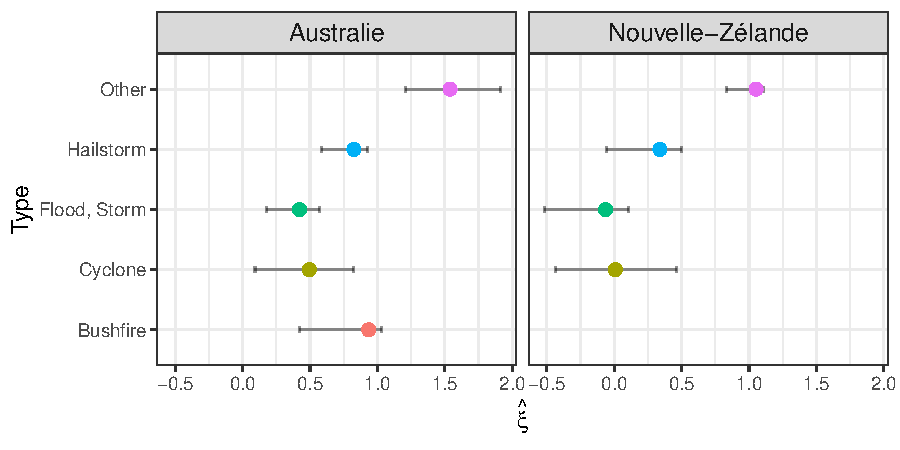
\includegraphics{images/fig-026}
\end{center}
\caption{Prédictions du paramètre $\xi$ avec intervalles de confiance à 95\%}
\label{fig:3.14}
\end{figure}

La figure \ref{fig:3.14} montre qu'il y a bel et bien une différence entre les différents types et que celle-ci est consirédablement importante. Ici, le comportement entre les types est semblable pour les deux pays, mais la figure montre clairement que les paramètres de l'Australie sont supérieurs à ceux de la Nouvelle-Zélande, ce qui est logique. De plus, contrairement aux résultats obtenus à la figure \ref{fig:3.8} où les résultats étaient non problématiques, les résultats obtenus ici contiennent deux valeurs (pour le même type) supérieures à 1, ce qui représente un modèle à moyenne infinie. Deux intervalles de confiance vont également jusqu'à des valeurs négatives sans toutefois atteindre -1, ce qui est très problématique.
\\

\begin{figure}[h]
\begin{center}
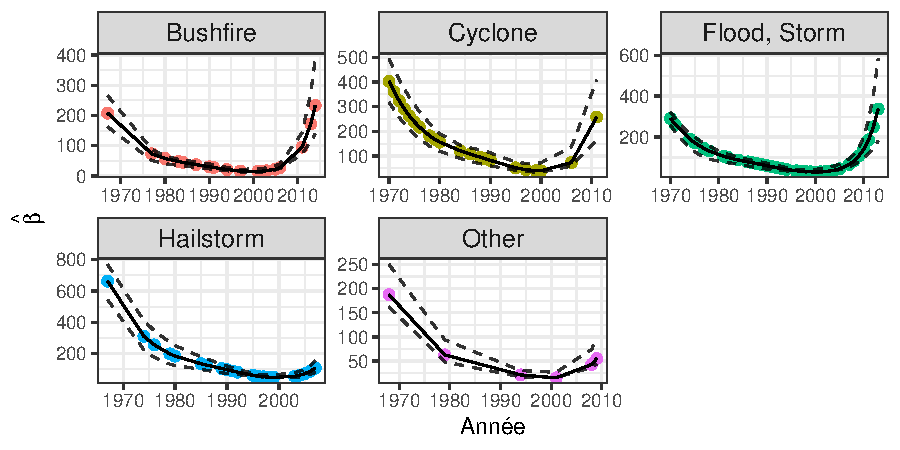
\includegraphics{images/fig-027}
\end{center}
\caption{Prédictions du paramètre $\beta$ pour l'Australie avec intervalles de confiance à 95\%}
\label{fig:3.15}
\end{figure}


\begin{figure}[h]
\begin{center}
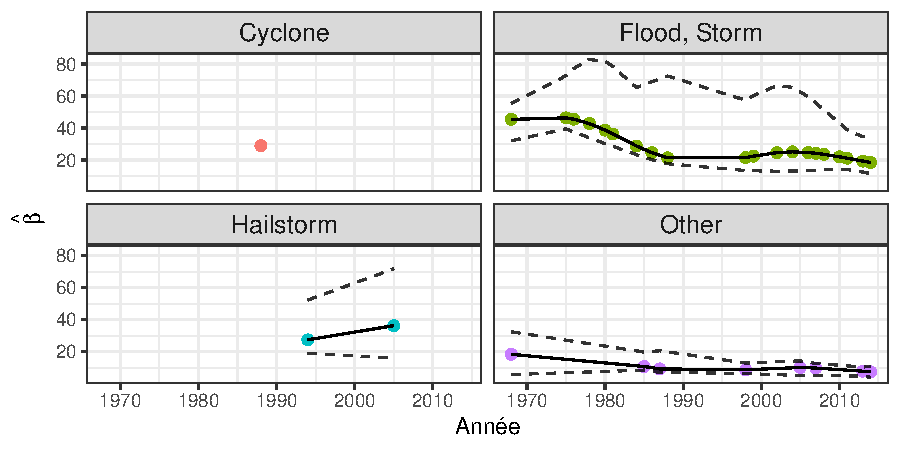
\includegraphics{images/fig-028}
\end{center}
\caption{Prédictions du paramètre $\beta$ pour la Nouvelle-Zélande avec intervalles de confiance à 95\%}
\label{fig:3.16}
\end{figure}

Les figures \ref{fig:3.15} et \ref{fig:3.16} montrent bien qu'encore une fois, le pays a une importance très significative pour la détermination des paramètres. De plus, même si cela est moins considérable que pour $\xi$, les figures montrent qu'il y a bel et bien une différence entre les différents types. Pour l'Australie, les courbes sont semblables, mais tout comme avec $\rho$, le type amène une certaine translation verticale de la courbe. Pour la Nouvelle-Zélande, le type amène également des courbes différentes. Un problème flagrant est remarquable à la figure \ref{fig:3.16} pour laquelle il y a très peu de points et donc des résultats peu crédibles. Ce problème est dû au fait qu'il y a déjà très peu de données et qu'en plus une troisième variable est rajoutée, ce qui rend les sous-groupes de covariables moins populés. Une autre cause vient du fait que seulement les données au-dessus du seuil $u$ sont utilisées pour la modélisation et la Nouvelle-Zélande présente beaucoup moins de pertes qui remplissent ce critère.
\\

Il est maintenant important de vérifier l'adéquation du modèle avant d'effectuer n'importe quelle inférence. Cette étape est également utile pour voir si l'ajout d'une troisième variable améliore le modèle. Le même type de graphique que la figure \ref{fig:3.10} est tracé à la figure \ref{fig:3.17}. 




\begin{figure}[h]
\begin{center}
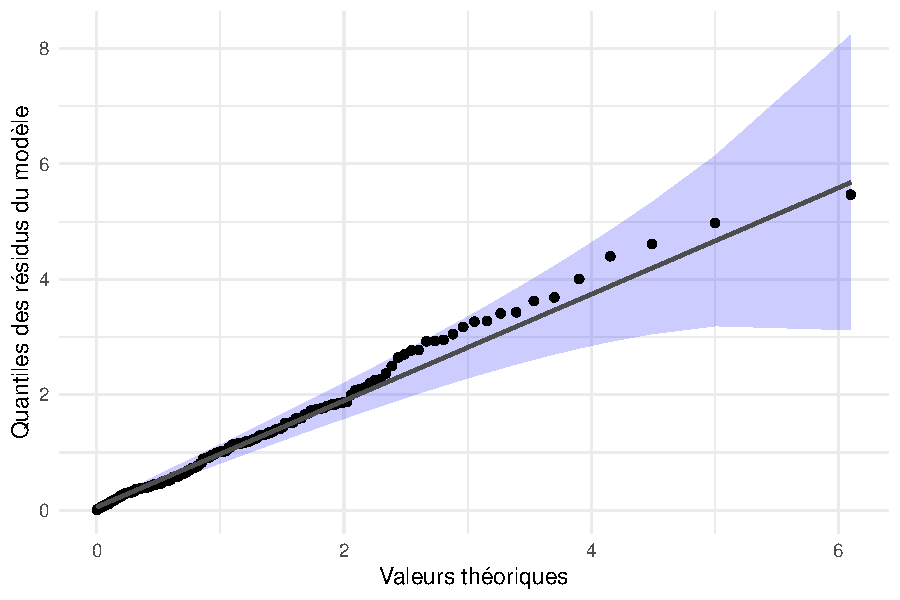
\includegraphics{images/fig-030}
\end{center}
\caption{Graphique \textit{Q-Q} de $\text{Exp}(1)$}
\label{fig:3.17}
\end{figure}

Le résultat obtenu à la figure \ref{fig:3.17} est, dans l'ensemble, très concluant, tout comme celui obtenu à la figure \ref{fig:3.10}. Il est difficile de dire lequel des graphiques est meilleur.


Les différentes $\widehat{\text{VaR}_{0.99}}$ peuvent maintenant être calculées. Les figures \ref{fig:3.18} et \ref{fig:3.19} montrent les résultats obtenus pour les deux pays. 
\begin{figure}[h]
\begin{center}
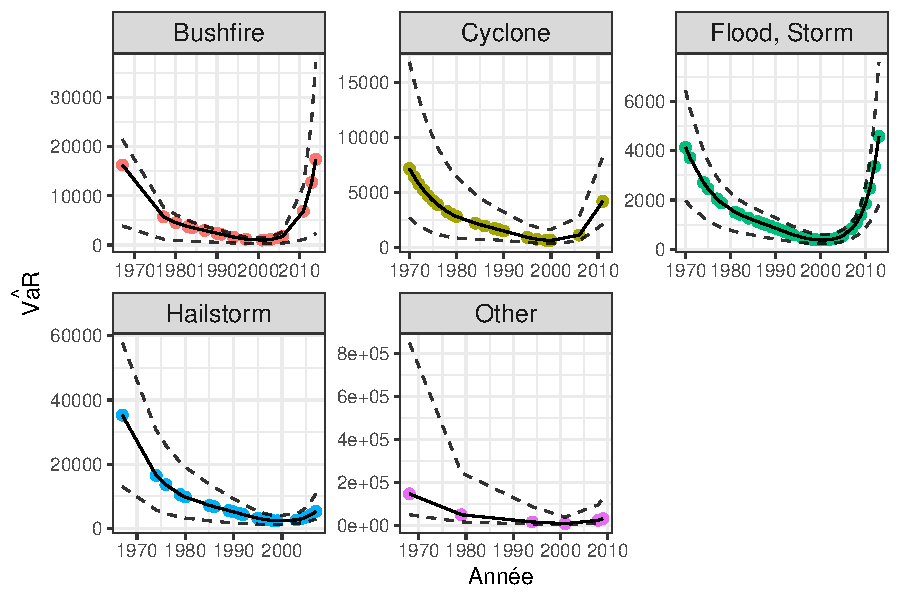
\includegraphics{images/fig-031}
\end{center}
\caption{$\widehat{\text{VaR}_{0.99}}$ avec intervalles de confiance à 95\%}
\label{fig:3.18}
\end{figure}

\begin{figure}[h]
\begin{center}
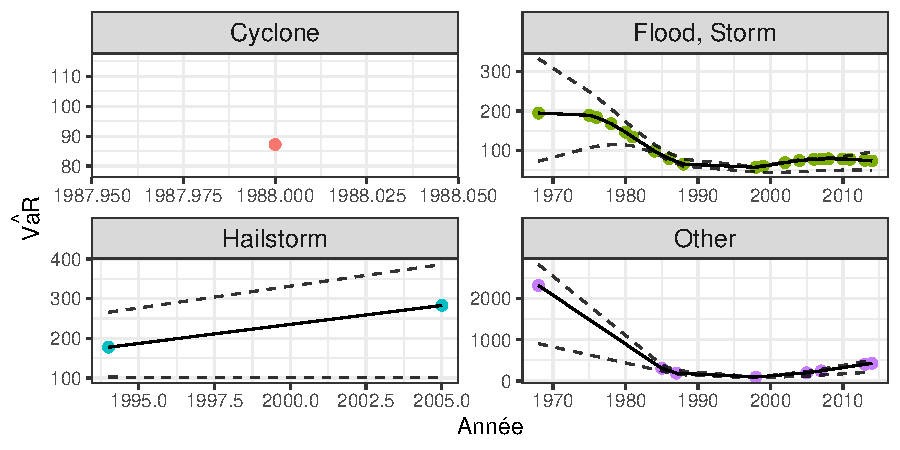
\includegraphics{images/fig-032}
\end{center}
\caption{$\widehat{\text{VaR}_{0.99}}$ avec intervalles de confiance à 95\%}
\label{fig:3.19}
\end{figure}

Tout comme à la section précédente, il est logique de voir que la mesure de risque dépend du temps, du type et du pays car celle-ci est obtenue avec les paramètres estimés et que les valeurs obtenues pour la Nouvelle-Zélande soient inférieurs que celles de l'Australie tout simplement parce que les pertes sont généralement plus élevées pour l'Australie.
\\

C'est ce qui conclut cette section. Cette section a montré que l'ajout d'une troisième variable catégorique est possible si celle-ci n'a pas trop de niveaux. Le modèle obtenu est adéquat, mais la qualité de celui-ci n'est pas grandement différente avec celle du modèle développé à la section \ref{sec:3.3} en plus que le modèle de la présente section présente des paramètres et des mesures de risques plus volatiles et moins crédibles. 
